\section{Background} \label{sec:background}

\subsection{KVM} \label{sec:kvm}

Fig 1 shows typical KVM architecture, with reference to a network related
application. 

\begin{figure}[t]
% \vspace{.20in}
\centering
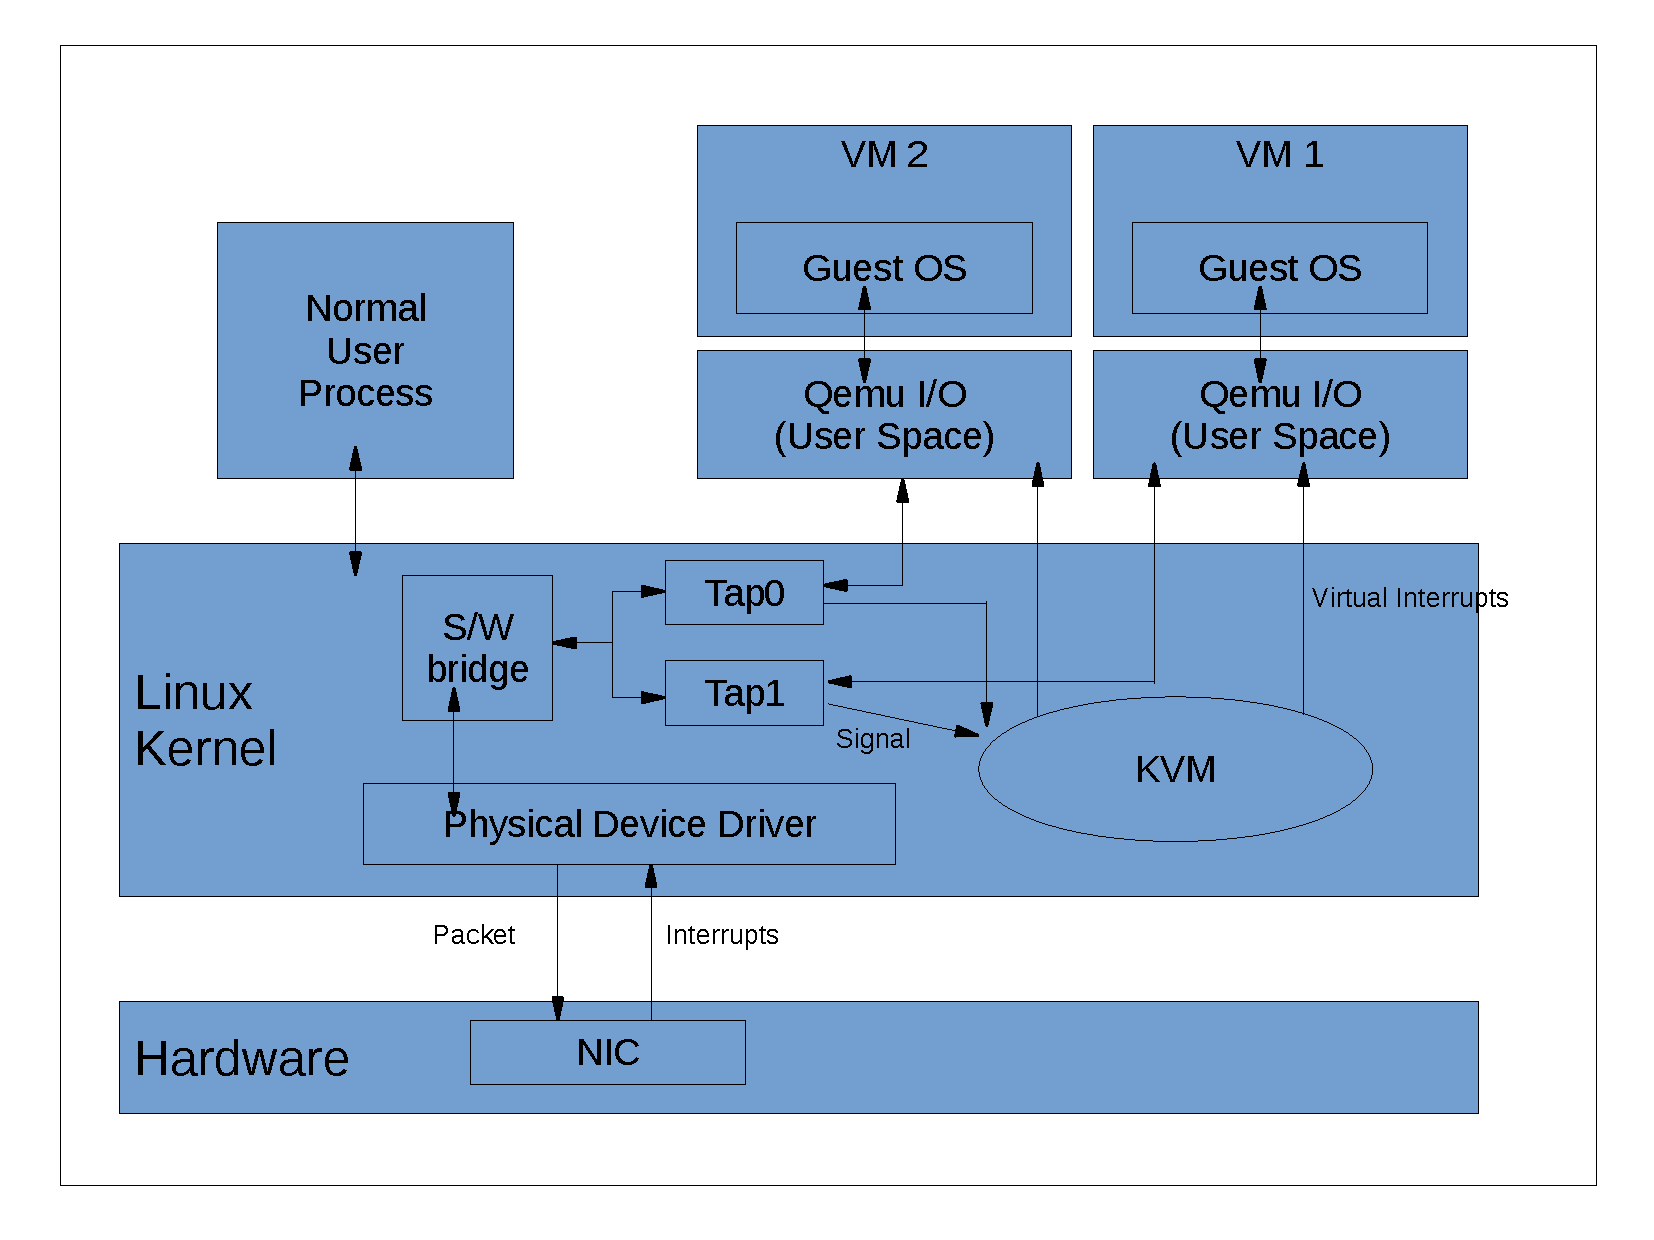
\includegraphics[width=.47\textwidth]{figures/kvm}
\vspace{-.2in}
\caption{{\em KVM Architecture.}} \label{fig:kvm}
\vspace{.05in}
\end{figure}

As depicted in the picture, when a packet arrives at physical NIC,
interrupts generated by NIC are handled by the physical device driver. The device
driver forwards the packet to software bridge. The bridge, then pushes the packet
to the tap device of the corresponding VM. The tap device is a virtual network
device that sends a signal to KVM module. KVM module in turn, generates a virtual
interrupt to the user space Qemu of the target VM. Qemu then copies the packet from
tap device and generates the interrupt for the guest OS emulating the virtual NIC.
Again, the physical device driver in the guest OS handles the packet transfer to
the VM’s address space. A major advantage of the KVM architecture is the full
availability of user-space tools in the QEMU process, such as threading, libraries
and so on.

\subsection{\paxos}\label{sec:paxos}

\subsection{RDMA} \label{sec:rdma}

\section{\xxx Overview} \label{sec:overview}

\subsection{Architecture} \label{sec:arch}

Figure 2 shows \xxx's architecture. It contains three main components.

\begin{figure}[t]
% \vspace{.20in}
\centering
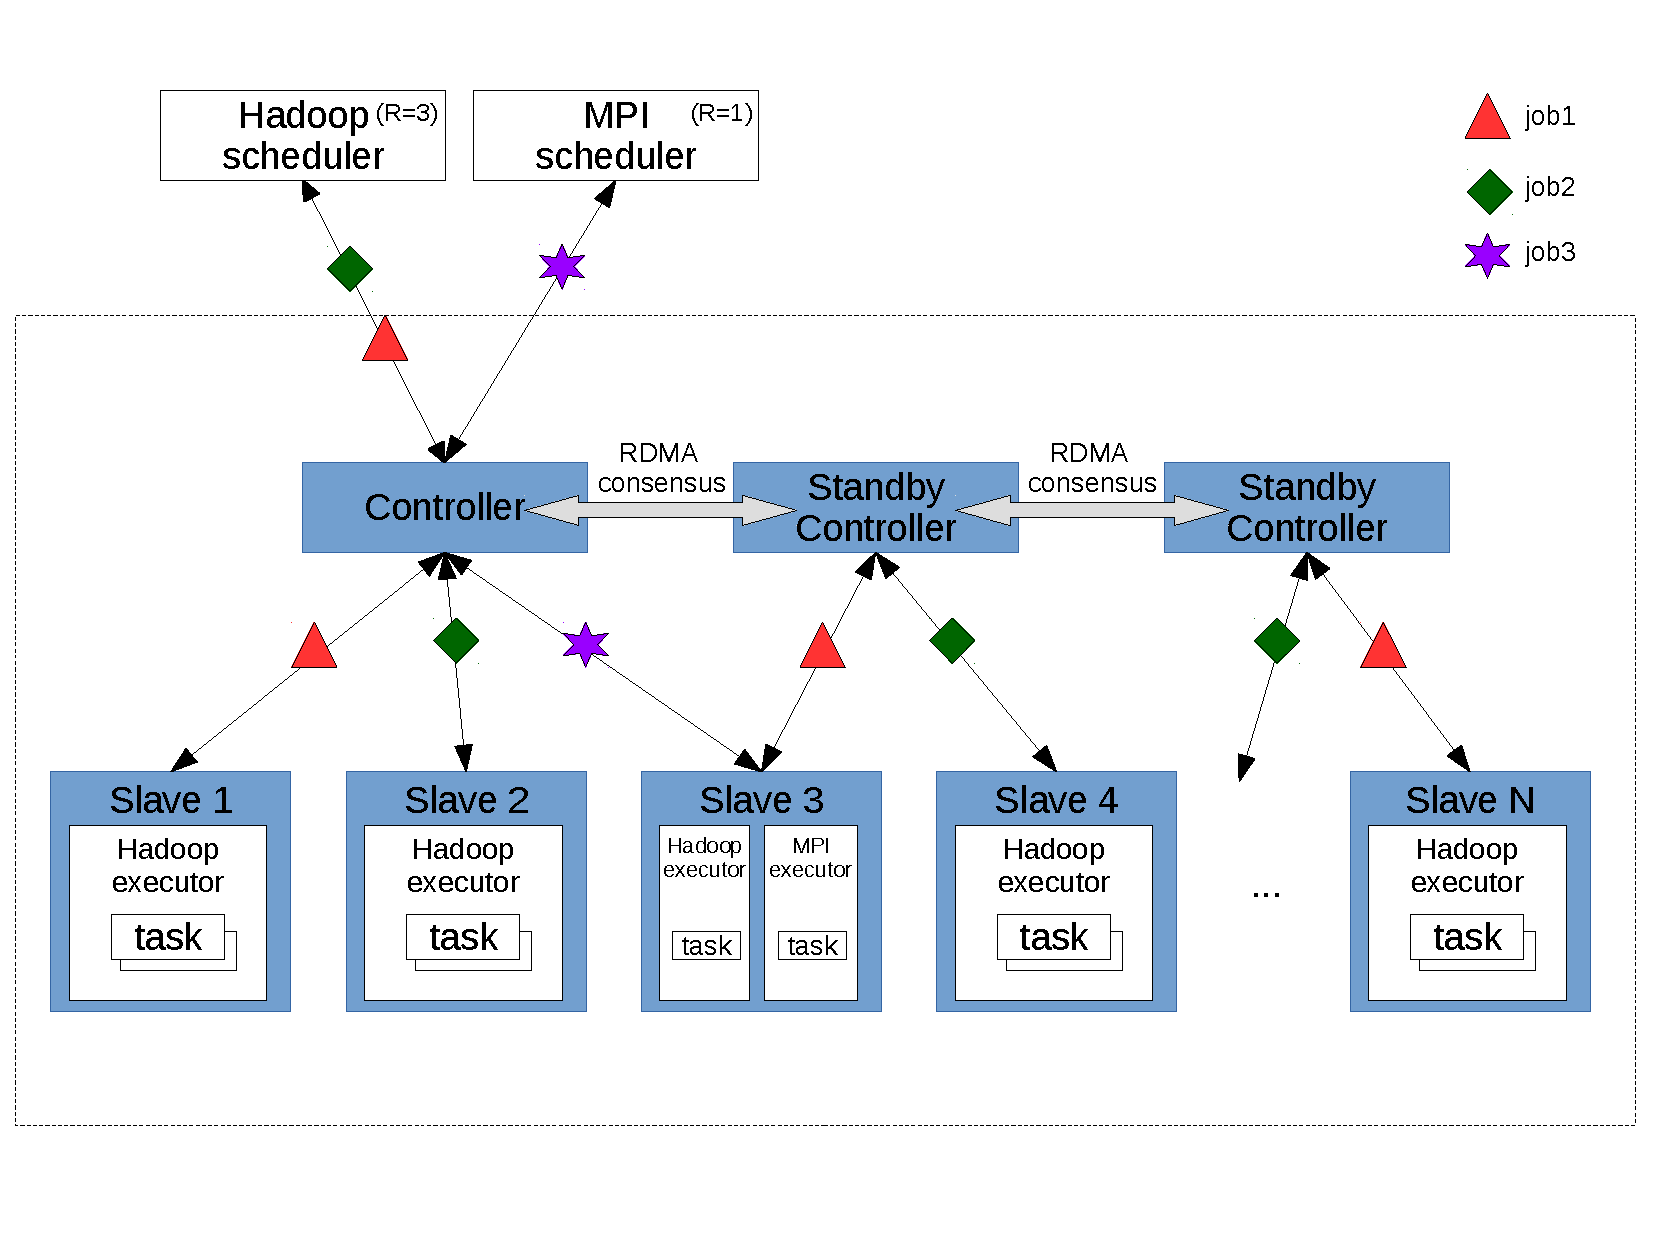
\includegraphics[width=.47\textwidth]{figures/arch}
\vspace{-.2in}
\caption{{\em The \xxx Architecture.}} \label{fig:arc}
\vspace{.05in}
\end{figure}

% On receiving a packet, QEMU calls tap_send()
% On sending a packet, QEMU calls tap_receive()
The replication logic is entirely implemented in qemu-kvm, a KVM tailored version of QEMU.
We maintain a packet queue to capture outgoing packets.
